\documentclass[a4paper, 12pt]{extarticle}
%\usepackage{ucs}
%\usepackage[utf8x]{inputenc}%[2014/04/30]         % Кодировка utf8
%Если будут проблемы со ссылками/библиографией, можно врубить ucs или utf8x
\usepackage[utf8]{inputenc}%[2014/04/30]         % Кодировка utf8
\usepackage[T2A]{fontenc}
\usepackage[english, russian]{babel}[2014/03/24]
%\usepackage{hyperref} 
\usepackage{amsmath}
\usepackage[left=2cm,right=2cm,
top=2cm,bottom=1.5cm,bindingoffset=0cm]{geometry}
\usepackage{ulem}
\usepackage{comment}
\usepackage{graphicx}
\usepackage{amssymb}
\usepackage{empheq}
\usepackage{fancybox,fancyhdr} %this packages provides fancy up and bottom of page
\fancyhead[R]{\footnotesize v0.1a}
\fancyhead[L]{\footnotesize Заготовка статьи по эффекту Фредерикса в ячейке ХЖК с учётом флекса при $\ve_a < 0$}
\def \q {{\bf q}}
\def \br {{\bf r}}
\def \k {{\bf k}}
\def \n {{\bf n}}
\def \ve {\varepsilon}
\def \vk {\varkappa}
\def \tz {\tilde{z}}
\def \ta {\tilde{a}}
\def \tc {\tilde{c}}
\def \tb {\tilde{b}}
\newcommand{\bb}[1]{\textbf{#1}}
\newcommand{\FF}{\mathcal{F}}
\renewcommand{\AA}{\mathcal{A}}
\newcommand{\BB}{\mathcal{B}}
\newcommand{\CC}{\mathcal{C}}
\newcommand{\DD}{\mathcal{D}}
\newcommand{\EE}{\mathcal{E}}
\newcommand{\II}{\mathcal{I}}
\begin{document}
\pagestyle{fancy}
\pagenumbering{arabic}%gobble}
\section{Постановка задачи}
Решается задача поиска устойчивой (стабильной) конфигурации ХЖК в плоскопараллельной ячейке, поле направлено перпендикулярно <<слоям>> ЖК, общий вид ячейки, а также обозначения углов $\theta$ и $\phi$ представлены на Рис.~\ref{pic_schematic_LC} и Рис.~\ref{pic_decart}.\par
\begin{figure}[ht!]
	\centering
	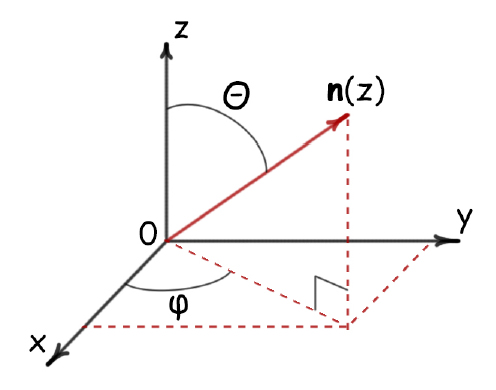
\includegraphics[width=10cm,keepaspectratio]{pic_04}
	\caption{Директор $\bb{n}(z)$ в сферическиз координатах $\theta(z)$ и $\phi(z)$}
	\label{pic_schematic_LC}
\end{figure}
\begin{figure}[ht!]
	\centering
	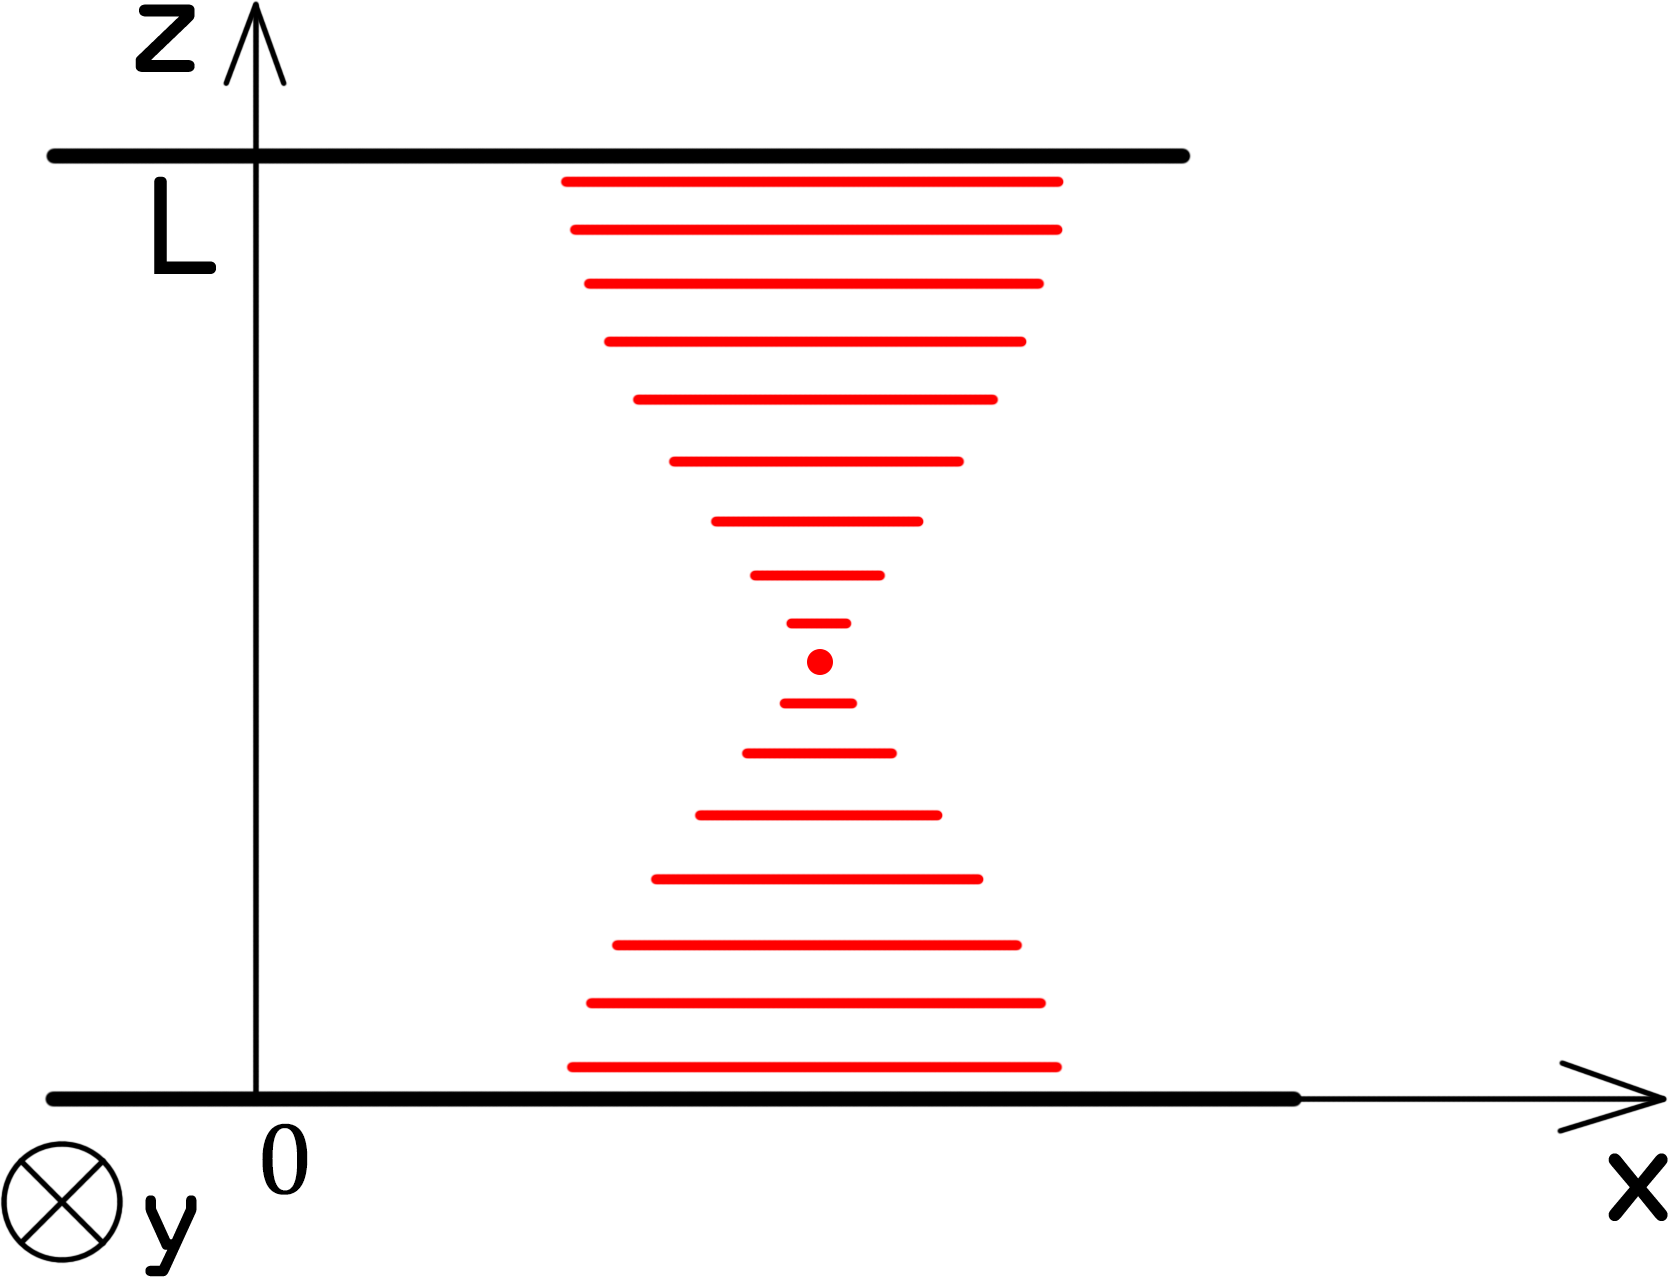
\includegraphics[width=10cm,keepaspectratio]{decart}
	\caption{Система координат, принятая в статье}
	\label{pic_decart}
\end{figure}
При этом выражение для свободной энергии имеет вид:
\begin{multline*}
\FF = \frac{S_\perp}{2}\Bigg[ -\frac{1}{4\pi}U^2 J + 2\bar{e}UJJ_1 + 4\pi \bar{e}^2\int\limits_{0}^{L} \frac{(\sin{(2\theta)}\theta' - JJ_1)^2}{\EE(\theta)}\ dz +\phantom{\Bigg]}\\
\phantom{\Bigg[}+ W_\theta^{(1)}\sin^2\left( \theta(0) - \theta_0^{(1)} \right) + W_\theta^{(2)}\left( \theta(L) - \theta_0^{(2)} \right) \Bigg]
\end{multline*}
Первая вариация свободной энергии может быть записана так (для удобства опустили у модулей граничной энергии значок $\theta$):
\begin{multline}\label{eq_dF_basic}
	\frac{\delta \FF}{S_\perp} = \left[-\frac{U^2 J^2}{8\pi} + \bar{e}UJ^2 J_1 + 2\pi\bar{e}^2\left( (y')^2 - 2y''y - J_1^2 J^2 \right)\right]\frac{\delta y(z)}{\ve_a y^2} +\\
	+ \left[ \bar{e}UJ - 4\pi \bar{e}^2\left(y'(0) + JJ_1\right)+\ve_a y(0) \frac{W_1}{2} \right]\frac{\delta y(0)}{\ve_a y(0)} +\\
	+\left[ -\bar{e}UJ + 4\pi \bar{e}^2\left(y'(L) + JJ_1\right)+\ve_a y(L) \frac{W_2}{2} \right]\frac{\delta y(L)}{\ve_a y(L)}.
\end{multline}
Наконец, условия на границе запишутся так:
\begin{eqnarray}
	&\left[-y'(0)-J\left(J_1-\frac{U}{4\pi\bar{e}}\right) + g_1 y(0)\right]\delta y(0) &\geqslant 0 \label{eq:border-left_basic}\\
	&\left[y'(L)+J\left(J_1-\frac{U}{4\pi\bar{e}}\right) + g_2 y(L)\right]\delta y(L) &\geqslant 0. \label{eq:border-right_basic}
\end{eqnarray}

\subsection{Преобразование задачи к удобному для решения виду}
Прежде чем перейти к рассмотрению возможных структур, преобразуем имеющиеся уравнения. В частности, отметим, что требование обнуления объёмного вклада в~\eqref{eq_dF_basic} приводит к дифференциальному уравнению второго порядка на $y(z)$, которое в общем случае имеет два решения -- линейное и параболическое. В предыдущей работе показано, что линейное решение не реализуется, а вот параболическое возникнуть может. Приведём его общий вид:
$$
y(z) = \frac{c}{4}(z+b)^2 - \frac{a^2}{c},
$$
причём оно является экстремалью функционала $\FF[y(z)]$ только если выполнено условие самосогласования
$$
a^2 = J^2\left(J_1 - \frac{U}{4\pi\bar{e}}\right)^2.
$$
Оказывается удобным перейти к безразмерным переменной и коэффициентам
\begin{eqnarray*}
	&\tc &\equiv -cL^2,\\
	&\ta &\equiv aL,\\
	&\tb &\equiv -b/L,\\
	&\tz &\equiv z/L.
\end{eqnarray*}
В этих терминах параболическое решение приобретает вид
$$
y(\tz) = \frac{\ta^2}{\tc} - \frac{\tc}{4}(\tz - \tb)^2, \quad \tz\in [0,\ 1]
$$

Задачу будем решать, находя и исследуя условия, при которых устойчивы следующие структуры, которые были найдены численной минимизацией в Матлабе -- они представлены на Рис.~\ref{pic_4_structures} и будут рассмотрены в соответствующем порядке.
\begin{figure}[ht!]
	\centering
	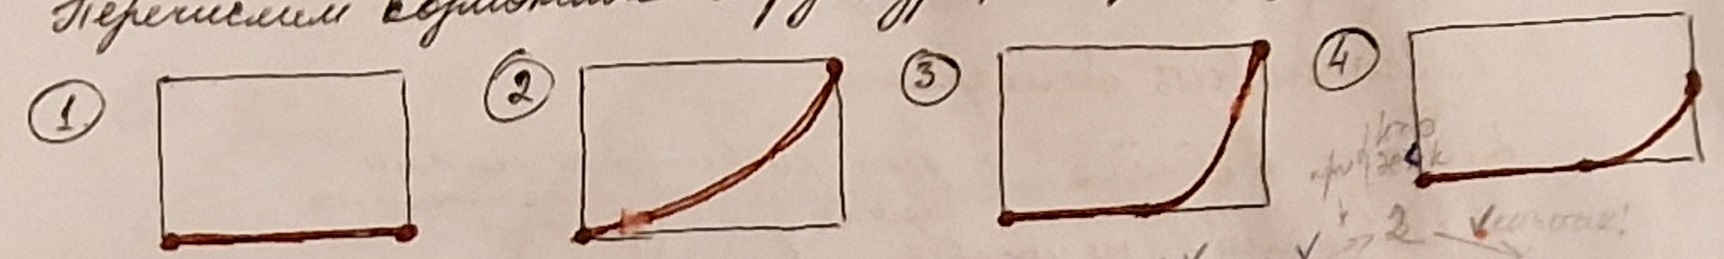
\includegraphics[width=17cm,keepaspectratio]{pic1}
	\caption{Возможные решения}
	\label{pic_4_structures}
\end{figure}


\section{Планарная структура}
\begin{figure}[ht!]
	\centering
	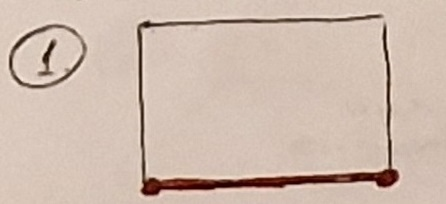
\includegraphics[width=10cm,keepaspectratio]{pic1a}
	\caption{Планарная структура}
\end{figure}
Уравнение известно, ничего находить не нужно:
$$
y(\tz) = \frac{\ve_\perp}{\ve_a} = -\vk^2,
$$
остаётся проверить следующие требования:
\begin{itemize}
	\item Устойчивость границ(справа и слева) -- по граничным условиям~\eqref{eq:border-left_basic} и~\eqref{eq:border-right_basic},
	\item устойчивость в объёме по неотрицательности первого (<<объёмного>>) слагаемого в выражении для первой вариации свободной энергии~\eqref{eq:border-left_basic}.
\end{itemize}
Выполняем проверку. На левой границе ($\tz = 0$) $\delta y(0) > 0$, $y' = 0$, и условие приобретает вид
$$
-J(J_1 - \frac{U}{4\pi\bar{e}}) - g_1\vk^2 \geqslant 0.
$$
Подставляя $J = \ve_\perp/L$ и $J_1 = 0$, получаем следующее неравенство:
$$
\frac{\bar{e}U}{L} + \frac{W_1}{2} \geqslant 0,
$$
которое верно всегда (с учётом того, что мы рассматриваем $U > 0$, поскольку отрицательные напряжения эквивалентны тому, что мы меняем границы местами).

Неравенство, выполнение которого необходимо для того, чтобы правая граница ($\tz = 1$) была устойчива, получается из условия~\eqref{eq:border-right_basic} аналогично:
$$
-\frac{\bar{e}U}{L} + \frac{W_2}{2} \geqslant 0.
$$
Соответственно, в терминах напряжений оно запишется как
\renewcommand{\theequation}{\arabic{equation}a}
\begin{equation}
	U \leqslant \frac{W_2 L}{2\bar{e}}.
\end{equation}
Для параметров $\gamma$ и $k$, определяемых соотношениями~\eqref{eq:appendix_gamma_definition} и~\eqref{eq:appendix_k_definition}, получаем
\addtocounter{equation}{-1}
\renewcommand{\theequation}{\arabic{equation}b}
\begin{equation}\label{eq:part1_final_cond}
	\gamma \leqslant \exp\left( \frac{1}{k+1}\right)
\end{equation}
\renewcommand{\theequation}{\arabic{equation}}


Наконец, проверим объём и для начала приведём само условие устойчивости:
$$
\left[-\frac{U^2 J^2}{8\pi} + \bar{e}UJ^2 J_1 + 2\pi\bar{e}^2\left( (y')^2 - 2y''y - J_1^2 J^2 \right)\right]\frac{\delta y(z)}{\ve_a y^2} \geqslant 0
$$
Внутри скобки все слагаемые, кроме первого, оказываются равными нулю, а дробь вне скобки -- отрицательная (поскольку $\delta y(z) > 0$, а $\ve_a < 0$).
Таким образом, получаем
$$
-\frac{U^2 \ve_\perp^2}{8\pi L^2} \leqslant 0,
$$
что верно всегда.

Таким образом, планарная структура разрушается по правой границе при нарушении условия~\eqref{eq:part1_final_cond}.


\section{Парабола из угла в угол}
\begin{figure}[ht!]
	\centering
	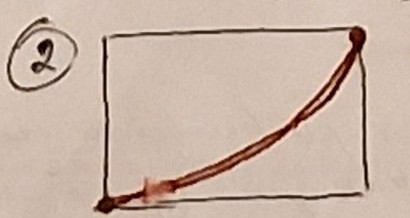
\includegraphics[width=10cm,keepaspectratio]{pic1b}
	\caption{Парабола, соединяющая два противоположных угла}
\end{figure}
Решение ищем в виде
\begin{equation}\label{eq:basic_function}
	y(\tz) = \frac{\ta^2}{\tc} - \frac{\tc}{4}(\tz - \tb)^2.
\end{equation}
Это одно из решений интегро-дифференциального уравнения второго порядка, которое возникает, если потребовать равенства нулю первой вариации свободной энергии $\FF_\mathrm{tot}$ в объёме.
Причём решением оно будет являться только при выполнении условия самосогласования:
\begin{equation}\label{eq:self-consistency}
\ta^2 = J^2L^2 \left( J_1 - \frac{U}{4\pi\bar{e}} \right)^2.
\end{equation}

В дальнейших расчётах понадобятся интегралы $J$ и $J_1$ (в приведённом расчёте для преобразования $J$ используется условие~\eqref{eq:geometry_part2}):
\begin{eqnarray}\label{eq:J_J1_calculated}
	&J_1 = \frac{1}{\ve_a}\ln\left(\frac{\vk^2}{\vk^2 - 1}\right)\\
	&J^{-1} = \frac{L}{\ve_a \ta}\ln\left| \frac{2\ta/\tc + 1 - \tb}{2\ta/\tc - \tb}\cdot\frac{2\ta/\tc + \tb}{2\ta/\tc - 1 + \tb} \right|.
\end{eqnarray}
Это выражение получено для параболического решения, идущего от края до края ячейки (без объёмных участков насыщения).

\subsection{Нахождение решения}
Начнём с выполнения требований геометрии решения:
\begin{equation}\label{eq:geometry_part2}
y(0) = -\vk^2,\quad y(1) = 1-\vk^2.
\end{equation}
Подставляя~\eqref{eq:basic_function} в~\eqref{eq:geometry_part2} и вычитая $y(0)$ из $y(1)$, получим следующую связь:
\begin{equation}
	\tb = \frac{4-\tc}{2\tc}.\label{eq:some_connection}
\end{equation}
С учётом этой связи, можно записать в удобной форме выражения для $y(0)$ и $y(1)$:
\begin{equation}
	\left\{
	\begin{aligned}
		(4-\tc-4\ta)(4-\tc+4\ta) &= -\vk^2 \cdot 16\tc\\
		(4+\tc-4\ta)(4+\tc+4\ta) &= (1 - \vk^2)\cdot 16\tc.
	\end{aligned}
	\right.\label{eq:ch2_some_eq}
\end{equation}
Далее проанализируем условия на границах~\eqref{eq:border-left_basic} и~\eqref{eq:border-right_basic}.
Учитывая, что в рассматриваемой конфигурации $\delta y(0) > 0$, а $\delta y(1) < 0$, можно записать:
\begin{eqnarray}
	&-y'(0) - J\left(J_1 - \frac{U}{4\pi\bar{e}}\right) + g_1 y(0) &\geqslant 0,\\
	&y'(L) + J\left(J_1 - \frac{U}{4\pi\bar{e}}\right) + g_2 y(L) &\leqslant 0.
\end{eqnarray}

Отметим, что в условии самосогласования~\eqref{eq:self-consistency} можно извлечь корень, и тогда возникает знак <<$\pm$>>:
\begin{equation}\label{eq:a_plus_minus}
	\ta = \pm JL \left( J_1 - \frac{U}{4\pi\bar{e}} \right).	
\end{equation}

Далее подставим в эти граничные условия функцию вида~\eqref{eq:basic_function} и учтём указанное выше соотношение для $\ta$. Получим:

\begin{eqnarray}
	&4-\tc \pm 4\ta+4g_1L\vk^2\leqslant 0 \label{eq:Lborder_ready}\\
	&4+\tc \pm 4\ta + 4g_1L(1-\vk^2)\leqslant 0 \label{eq:Rborder_ready}
\end{eqnarray}
для случая $\ta < 0$, то есть при знаке <<$+$>> в~\eqref{eq:a_plus_minus}. При знаке <<$-$>> получаем:
\begin{eqnarray}
	&4 - \tc - 4\ta + 4g_1L\vk^2\leqslant 0\\
	&4 + \tc - 4\ta + 4g_1L(1-\vk^2)\leqslant 0.
\end{eqnarray}


\iffalse
Как и ожидалось, выбор знака влияет только на знак $\ta$, причём в выражении для функции $y(\tz)$ стоит $\ta^2$, так что знак на физику влиять не должен.
Проверим, так ли это. Полученные неравенства для границ отличаются знаками в некоторых слагаемых.
Можно увидеть, что при выборе $\ta > 0$ получается <<$+4\ta$>>, а при выборе $\ta < 0$ получается <<$-4\ta$>>.
Таким образом, это слагаемое в обеих версиях неравенств просто должно быть положительным -- а значит, эти две версии системы неравенств эквивалентны.

Таким образом, можно просто выбрать один из знаков в выражении для $\ta$. Выберем <<$+$>>:
\begin{equation}\label{eq:a_plus}
	\ta = JL \left( J_1 - \frac{U}{4\pi\bar{e}} \right).	
\end{equation}
\fi
Подставим в условие самосогласования~\eqref{eq:a_plus_minus} подсчитанные ранее интегралы~\eqref{eq:J_J1_calculated}
После несложных преобразований получим для $\ta < 0$, знак <<$+$>> в~\eqref{eq:a_plus_minus}:
\begin{equation}
	\ln{\left| \frac{4\ta+4-\tc}{4\ta+4+\tc} \right|} = \ln{\left( \frac{\vk^2}{\vk^2 - 1}\right)} - \frac{\ve_a U}{8\pi \bar{e}},
\end{equation}
что можно переписать в виде
\begin{equation}
	\left| \frac{4\ta+4-\tc}{4\ta+4+\tc}  \right| = \frac{\vk^2}{\vk^2 - 1}\cdot\gamma.\label{eq:gammaSig1}
\end{equation}

Для $a>0$ (знака <<$-$>> в~\eqref{eq:a_plus_minus}) можно по аналогии получить:
\begin{equation}
	\left| \frac{4\ta+4-\tc}{4\ta+4+\tc}  \right| = \frac{1}{\gamma}.\label{eq:gammaSign2}
\end{equation}
Отметим, что при раскрытии модулей в полученных уравнениях~\eqref{eq:gammaSign2} и~\eqref{eq:gammaSign2} ещё раз возникает знак <<$\pm$>>.
При решении каждого из полученных уравнений совместно с~\eqref{eq:ch2_some_eq}, можно получить следующие выражения для коэффициентов, причём результат оказывается не зависящим от выбора знака в~\eqref{eq:a_plus_minus}, в то время как разный знак при раскрытии модуля в~\eqref{eq:gammaSign2} (или~\eqref{eq:gammaSign2}) приводит к двум разным решениям:
\begin{eqnarray}\label{eq:ch3_coeffs1_a}
	&\ta &= -1 + \frac{1-\gamma}{\gamma}\left( \vk^2(1+\gamma) - 1 \right)\\
	\label{eq:ch3_coeffs1_b}
	&\tb &= \frac{1}{2}\cdot\frac{\gamma}{1 - \gamma}\cdot\frac{1}{\vk^2(1 - \gamma) -1 } - \frac{1}{2}\\
	\label{eq:ch3_coeffs1_c}
	&\tc &= 4\cdot\frac{1 - \gamma}{\gamma}\cdot\left(\vk^2(1 - \gamma) - 1 \right)
\end{eqnarray}
для модуля, раскрытого со знаком <<$+$>> и
\begin{eqnarray}\label{eq:ch3_coeffs2_a}
	&\ta &= -1 - \frac{1+\gamma}{\gamma}\left( \vk^2(1+\gamma) - 1 \right)\\
	\label{eq:ch3_coeffs2_b}
	&\tb &= -\frac{1}{2}\cdot\frac{\gamma}{\gamma + 1}\cdot\frac{1}{\vk^2(1 + \gamma) -1 } - \frac{1}{2}\\
	\label{eq:ch3_coeffs2_c}
	&\tc &= -4\cdot\frac{1 + \gamma}{\gamma}\cdot\left(\vk^2(1 +
	 \gamma) - 1 \right)
\end{eqnarray}
для знака <<$-$>>.
Отметим, что один набор коэффициентов получается из другого заменой  $\gamma \to -\gamma$.
Для того, чтобы более удобно ссылаться на эти решения, обозначим набор~\eqref{eq:ch3_coeffs1_a}~--~\eqref{eq:ch3_coeffs1_c} как <<$+\gamma$>>, а~\eqref{eq:ch3_coeffs2_a}~--~\eqref{eq:ch3_coeffs2_c} как <<$-\gamma$>>.

\subsection{Проверка корректности решения}
Далее проверим корректность положения вершины параболы (это аналогично тому, что парабола целиком находится в заданном ограничениями <<прямоугольнике>> на плоскости $O\tz y$).
%и устойчивость границ (условия~\eqref{eq:Lborder_ready} и~\eqref{eq:Rborder_ready}).
Для того, чтобы парабола не выходила за границы прямоугольника, необходимо, чтобы вершина $\tz_\text{в}$ лежала вне диапазона $(0;1)$.


\subsubsection{Случай <<$-\gamma$>>}
Начнём с проверки положения вершины для случая <<$-\gamma$>>. 

Требование:
$$
\left[
\begin{aligned}
	&\tz_\text{в} \leqslant 0,\\
	&\tz_\text{в} \geqslant 1,
\end{aligned}
\right.
$$
координата вершины даётся выражением
$$
\tz_\text{в} = -\tb = \frac{1}{2} - \frac{\gamma}{1 + \gamma}\cdot\frac{1}{2\left( 1 - \vk^2(1 + \gamma) \right)}
$$
Подстановка этого выражения в условие $\tz_\text{в}\leqslant 0$ приводит к следующему неравенству:
\begin{equation}
	1 \leqslant \frac{\gamma}{(1+\gamma)(1-\vk^2(1+\gamma))}.
\end{equation}
Учитывая, что $\gamma > 1$ и $\vk > 1$, делаем вывод, что правая часть в полученном неравенстве $<0$.
Таким образом, решений нет.

Обратимся ко второму возможному условию, $\tz_\text{в} \geqslant 1$.
Оно приводит нас к следующему неравенству:
$$
\frac{\gamma}{(1+\gamma)(1 - \vk^2(1+\gamma))} \leqslant -1.
$$
Заметим, что знаменатель левой части неравенства $< 0$.
Преобразуя это неравенство, можно получить следующее выражение:
$$
\vk^2(1+\gamma)^2 - 2(1+\gamma) + 1 \leqslant 0.
$$
При этом левая часть неравенства может быть оценена следующим образом (поскольку $\vk > 1$):
$$
\vk^2(1+\gamma)^2 - 2(1+\gamma) + 1 \geqslant (1+\gamma)^2 - 2(1+\gamma) + 1 > 1,
$$
а значит, решений в данном случае нет.

\subsubsection{Случай <<$+\gamma$>>}
Аналогичным образом рассмотрим возможные допустимые положения вершины в случае знака <<$+\gamma$>>
В данном случае координата вершины даётся выражением
$$
\tz_\text{в} = -\tb = \frac{1}{2} - \frac{\gamma}{1 - \gamma}\cdot\frac{1}{2\left( \vk^2(1 - \gamma) -1 \right)}.
$$
Условие $\tz_\text{в} \leqslant 0$ приводит к следующему неравенству:
$$
1 \leqslant \frac{\gamma}{(1-\gamma)(\vk^2(1-\gamma)-1)}
$$
Трансформируя выражение (знаменатель дроби справа положительный), получим содержательное неравенство:
\begin{equation}\label{eq:condition_plusgamma_correct_align}
	\gamma \leqslant 1 + \frac{1}{\vk}.
\end{equation}
При соблюдении этого требования вершина параболы расположена левее интервала $[0, 1]$. 

Проверим второе возможное условие, $\tz_\text{в} \geqslant 1$:
$$
\frac{\gamma}{(\gamma-1)(\vk^2(1-\gamma)-1)} \geqslant 1
$$
В этом случае знаменатель дроби слева (а значит, и вся дробь) отрицателен, следовательно, решений нет.

Таким образом, условию на вершину удовлетворяют только решения, полученные при раскрытии модуля через <<$+\gamma$>>.
Кроме того, для корректности решения необходимо выполнение неравенства~\eqref{eq:condition_plusgamma_correct_align}.

\subsection{Устойчивость решения на границах}
Для того, чтобы решение было устойчивым на границе, необходимо выполнение граничных условий (неравенств)~\eqref{eq:border-left_basic} и~\eqref{eq:border-right_basic}. Учтём, что $\delta y(0) \geqslant 0$, $y(0) = -\vk^2$, $y'(0) = \tc/2$, и соберём условие на \underbar{левой границе}~\eqref{eq:border-left_basic}.
$$
-\frac{2}{L}\times\frac{1-\gamma}{\gamma}\times(\vk^2(1-\gamma) - 1)\times\left( -\frac{1}{2} + \frac{\gamma}{1-\gamma}\cdot\frac{1}{2(\vk^2(1-\gamma)-1)} \right) - \frac{\vk^2(1-\gamma^2)-1}{\gamma L} - g_1\vk^2 \geqslant 0.
$$
Отметим, что в первом слагаемом появился множитель $1/L$.
Это произошло из-за того, что в производной должна быть сделана замена переменной: $dy/dz = dy/d\tz\cdot\tz'_z = dy/d\tz\cdot L^{-1}$.
После преобразований можно получить следующее простое неравенство:
$$
\gamma \geqslant 1 + \frac{g_1 L}{2},
$$
что оказывается верным всегда, поскольку $\gamma > 1$, а $g_1 < 0$ (т.к. в него входит $\ve_a < 0$, см. Приложение 1).

Проанализируем устойчивость на правой границе, $\tz = 1$.
Здесь стоит учесть, что $\delta y(1) \leqslant 0$, $y(1) = 1 - \vk^2$, $y'(1) = \tc(1+\tb)/2$.
В результате условие на \underbar{правой границе}~\eqref{eq:border-right_basic} запишется так:
$$
\frac{2}{L}\times\frac{1-\gamma}{\gamma}\times(\vk^2(1-\gamma) - 1)\times\left( \frac{1}{2} + \frac{\gamma}{1-\gamma}\cdot\frac{1}{2(\vk^2(1-\gamma)-1)} \right) + \frac{\vk^2(1-\gamma^2)-1}{\gamma L} + g_2(1-\vk^2) \leqslant 0.
$$
Это выражение сводится к следующему неравенству:
$$
\gamma\left( 1+\frac{g_2 L}{2} \right) \geqslant 1.
$$
В дальнейшем удобно ввести параметр $\kappa$, связанный с модулем сцепления с правой границей:
$$
\kappa = -\frac{2}{g_2 L} - 1,
$$
в терминах $\kappa$ неравенство приобретает вид
$$
\gamma\cdot\frac{\kappa}{\kappa+1} \geqslant 1.
$$
Отметим, что параметр $\kappa \in (-1; +\infty)$.
При этом малые значения параметра соответствуют сильному сцеплению с границей, большие -- слабому.
Далее возможны два варианта:
\begin{enumerate}
	\item Если $-1 < \kappa < 0$, то решений нет. 
	Это соответствует <<сильному сцеплению>> на правой границе;
	\item Если же $\kappa >0$ (<<слабое сцепление>>), то правая граница будет устойчива при
	$$
	\gamma \geqslant 1 + \frac{1}{\kappa}.
	$$
	Отметим, что это условие содержательное и выполняется при напряжении, превосходящем некоторое критическое значение ($\gamma$ растёт вместе с $U$).
\end{enumerate}

\subsection{Результаы}
Решение типа <<парабола из угла в угол>> возможно и существует при выполнении следующих условий (при этом его коэффициенты даются уравнениями~\eqref{eq:ch3_coeffs1_a},~\eqref{eq:ch3_coeffs1_b} и~\eqref{eq:ch3_coeffs1_c}.):
\begin{itemize}
	\item На левой границе условие устойчивости всегда выполнено;
	\item Если сцепление с правой границей слишком сильное, то решений нет.
	Управляющее неравенство (условие на модуль сцепления):
	$$
	\kappa > 0.
	$$
	Если это условие выполнено, то граница устойчива при
	$$
	\gamma \geqslant 1+\frac{1}{\kappa};
	$$
	\item Чтобы вершина параболы не оказалась на интервале $[0,1]$, требуется выполнение следующего условия:
	$$
	\gamma < 1+\frac{1}{\vk}.
	$$
\end{itemize}
Таким образом, параметр $\gamma$, прямо зависящий от напряжения $U$, оказывается ограничен сверху и снизу:
$$
1+\frac{1}{\kappa} \leqslant \gamma \leqslant 1 + \frac{1}{\vk}.
$$
Очевидно, это имеет смысл при
$$
\kappa > \vk.
$$
Отметим, что реализации этого решения способствует слабая анизотропия диэлектрической проницаемости ЖК и слабое сцепление с правой границей.
\hrule

\section{Парабола с насыщением и закреплёнными концами}

\begin{figure}[ht!]
	\centering
	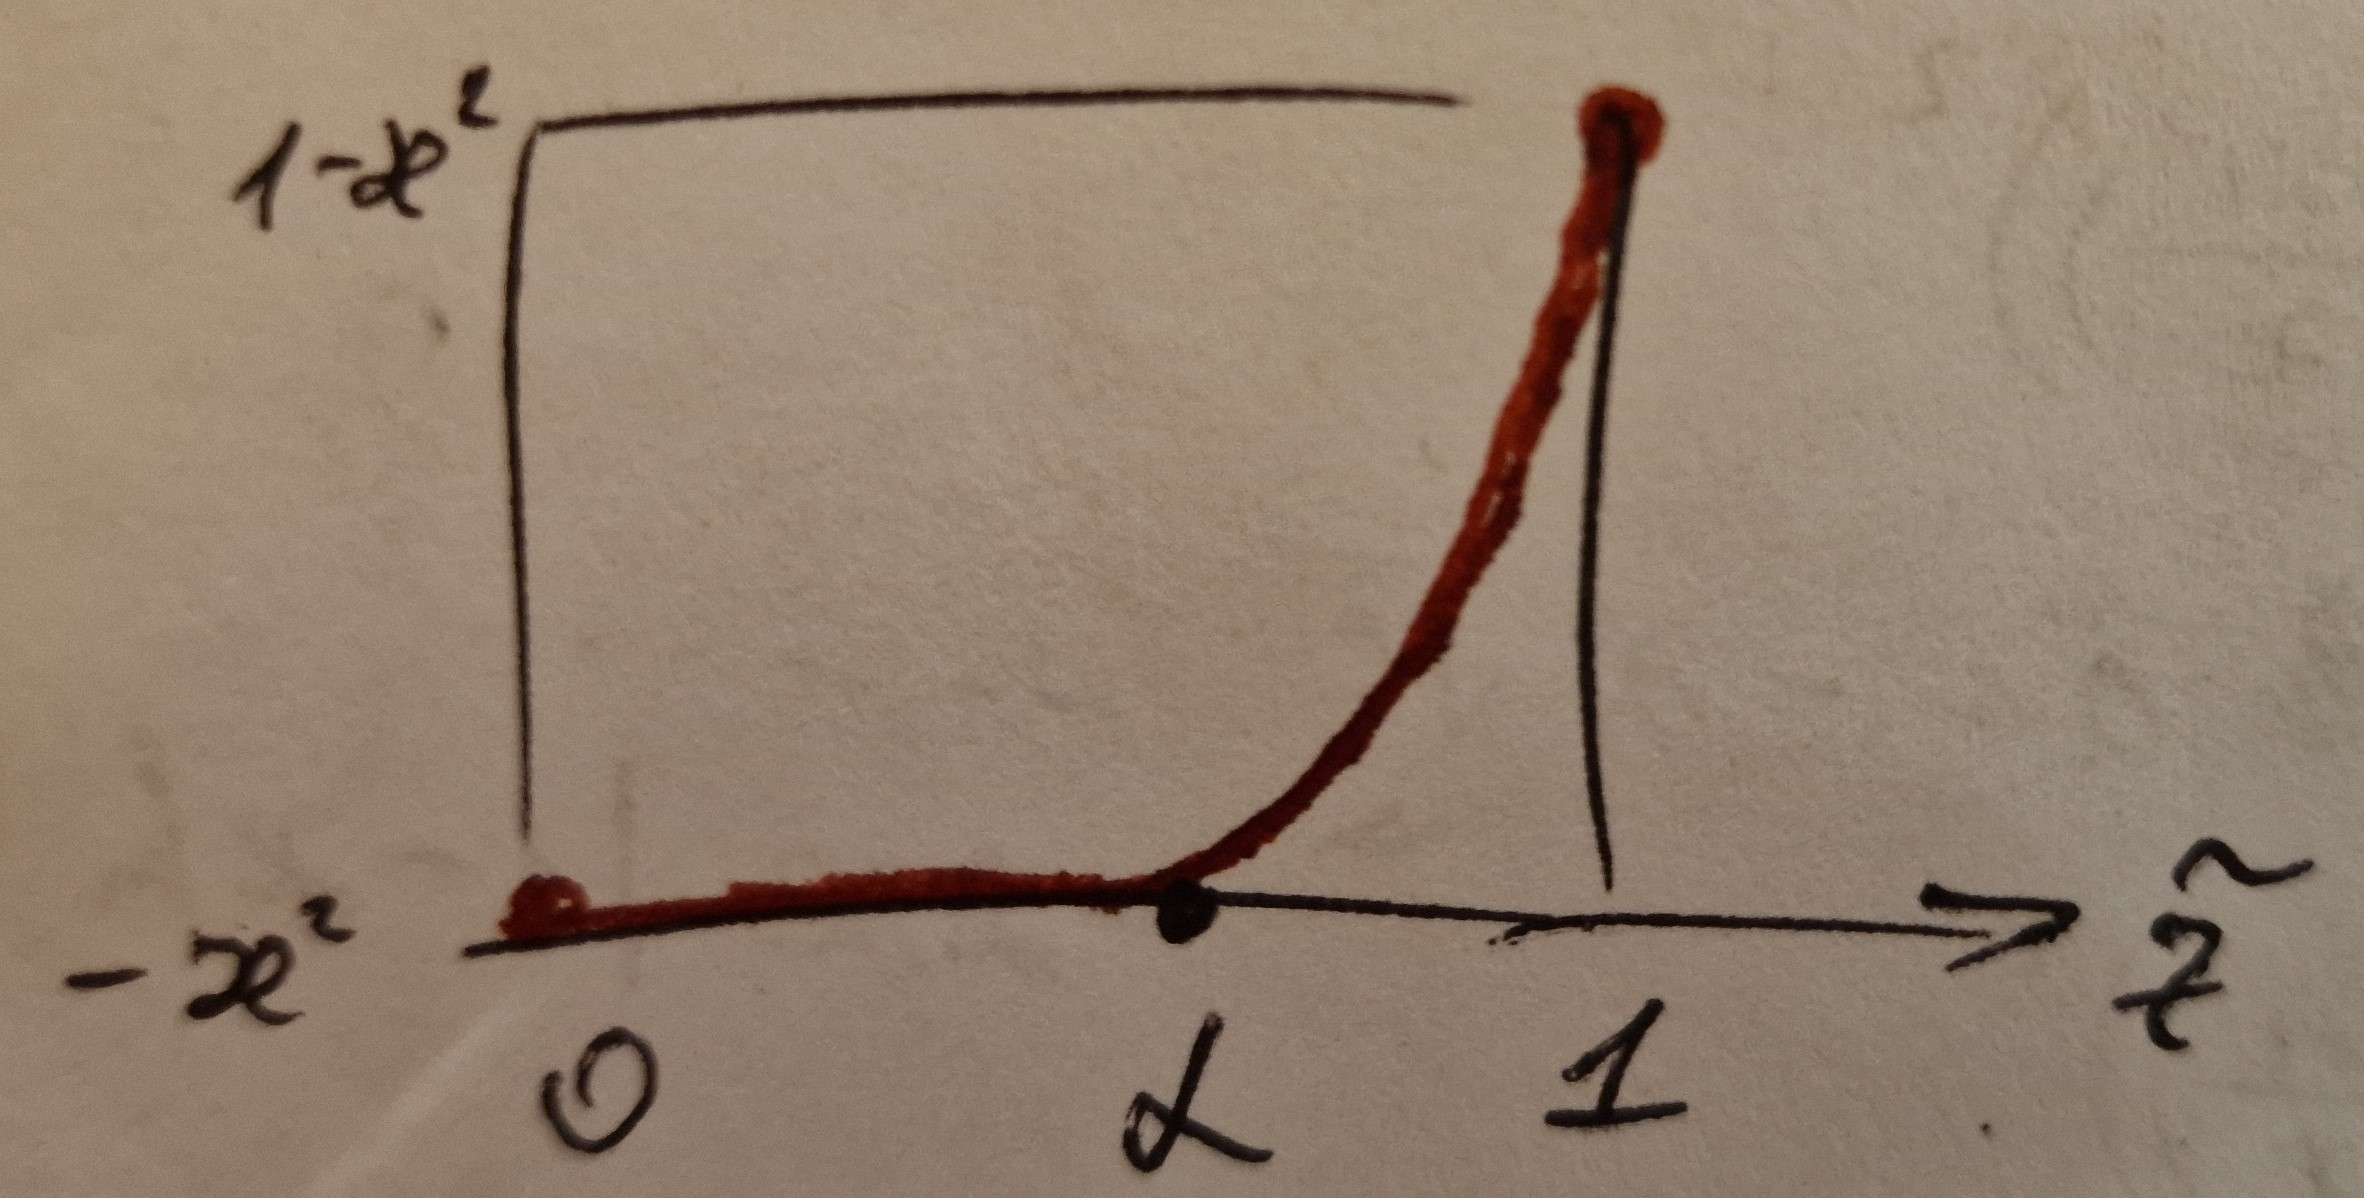
\includegraphics[width=10cm,keepaspectratio]{pic1c}
	\caption{Парабола с насыщением, соединяющая два противоположных угла}
\end{figure}

Решение будем искать в виде
\begin{equation}\label{eq:ch4_general}
	y(\tz) = \left\{
	\begin{aligned}
		&-\vk^2, &\tz\in [0,\alpha]\\
		&\frac{\tc}{4}\left(\tz + \tb\right)^2 - \frac{\ta^2}{\tc}, &\tz\in [\alpha, 1]
	\end{aligned}
	\right.
\end{equation}

Нужно, чтобы решение удовлетворяло следующим требованиям:
\begin{enumerate}
	\item Геометрические:
	\begin{equation}\label{eq:ch4_geometry}
		\left\{
		\begin{aligned}
			&y(\alpha+0) = -\vk^2,\\
			&\tz_\text{в} = \alpha,\\
			&y(1) = 1-\vk^2.
		\end{aligned}
		\right.
	\end{equation}
	\item Физические (устойчивость границ и самосогласование):
	\begin{equation*}
		\left\{
		\begin{aligned}
			&\text{неравенства на границе},\\
			&\ta^2 = J^2 L^2 \left(J_1 - \frac{U}{4\pi\bar{e}}\right)^2
		\end{aligned}
		\right.
	\end{equation*}
	\item Корректность положения вершины параболы:
	$$
	\alpha\in[0,1]
	$$
\end{enumerate}
\subsection{Нахождение решения}
Для начала подставим искомую функцию~\eqref{eq:ch4_general} в геометрические условия~\eqref{eq:ch4_geometry}:
\begin{equation}
\left\{
\begin{aligned}
	&\frac{\tc}{4}(\alpha + \tb)^2 - \frac{\ta^2}{\tc} = -\vk^2,\\
	&\tz_\text{в} = -\tb = \alpha\\
	&\frac{\tc}{4}(1 + \tb)^2 - \frac{\ta^2}{\tc} = 1-\vk^2.
\end{aligned}
\right.
\end{equation}
В результате можно получить следующие сязи (предлагается всё выразить через $\tb$, а затем найти её через условие самосогласования):
\begin{empheq}[left=\empheqlbrace]{align}
	&\tb = -\alpha,\label{eq:ch4_alpha_and_b_connection}\\
	&\tc = \frac{4}{(1-\alpha)^2},\label{eq:ch4_c_and_alpha_connection}\\
	&\ta^2 = \frac{4\vk^2}{(1-\alpha)^2}.\label{eq:ch4_a_and_alpha_connection}
\end{empheq}
Заметим, что $\tc > 0$ -- это также необходимо для того, чтобы парабола располагалась корректно.
\hrule

Для работы с условием самосогласования необходимо взять интегралы $J$ и $J_1$:
\begin{alignat}{2}
	&J_1 &&= \frac{1}{\ve_a}\ln{\frac{y(0)}{y(1)}} = \ve_a^{-1} \ln{\left( \frac{\vk^2}{\vk^2-1} \right)}\label{eq:ch4_J1_straight}\\
	&J^{-1} &&= \ve_a^{-1}L\int\limits_0^{1} \frac{d\tz}{y(\tz)} = \frac{L\tb}{\ve_a\vk^2} + \frac{L(1+\tb)}{2\ve_a\vk}\cdot \ln{\left( \frac{\vk-1}{\vk+1} \right)}\label{eq:ch4_J_straight}
\end{alignat}

Снимая квадрат в условии самосогласования, получим
\begin{equation}
J_1 - \frac{U}{4\pi\bar{e}} = \frac{\pm \ta J^{-1}}{L}.\label{eq:ch4_self-consistency_final}
\end{equation}
Отметим, что выражение слева отрицательно, а интеграл $J$ положителен.
Таким образом, какой бы знак в выражении $\pm\ta$ мы ни выбрали, само это выражение должно быть отрицательно.
Воспользовавшись связью~\eqref{eq:ch4_a_and_alpha_connection}, заменим
$$
\pm a \to \frac{-2\vk}{1-\alpha}.
$$
С учётом этого замечания, условие самосогласования~\eqref{eq:ch4_self-consistency_final} приводит нас к выражению для $\alpha$:
\begin{equation}
	\alpha = \frac{\vk\ln{\left(\frac{\gamma\vk}{\vk+1}\right)}}{1+\vk\ln{\left(\frac{\gamma\vk}{\vk+1}\right)}}.\label{eq:ch4_alpha_result}
\end{equation} 

С помощью связей~\eqref{eq:ch4_alpha_and_b_connection},~\eqref{eq:ch4_c_and_alpha_connection} и~\eqref{eq:ch4_a_and_alpha_connection} можно найти коэффициенты $\tc$, $\ta^2$ (для удобства записи функции $y(\tz)$ запишем именно в квадрате) и $\alpha$ соответственно:
\begin{alignat}{2}
	&\tc &&= 4\left(1+\vk\ln{\left(\frac{\gamma\vk}{\vk+1}\right)}\right)^2,\\
	&\alpha &&= \frac{\vk\ln{\left(\frac{\gamma\vk}{\vk+1}\right)}}{1+\vk\ln{\left(\frac{\gamma\vk}{\vk+1}\right)}},\\
	&\ta^2 &&= \frac{4\vk^2}{(1-\alpha)^2}.	
\end{alignat}
Сама же функция $y(\tz)$ запишется так:
\begin{equation}\label{eq:ch4_general_2}
	y(\tz) = \left\{
	\begin{aligned}
		&-\vk^2, &\tz\in [0,\alpha]\\
		&\left( \frac{\tz-\alpha}{1-\alpha} \right)^2 - \vk^2, &\tz\in [\alpha, 1]
	\end{aligned}
	\right.
\end{equation}

\subsection{Проверка положения вершины}
\subsection{Проверка устойчивости на границах}


\newpage
\section*{Приложение 1. Список используемых обозначений}
Интегралы:
$$
J^{-1} = \frac{1}{\ve_a}\int\limits_0^{L} \frac{dz}{y(z)} = \frac{L}{\ve_a}\int\limits_{0}^{1} \frac{d\tz}{y(\tz)}
$$

\begin{alignat}{2}
	&\text{Преобразованные модули энергии на границах:} &&g_i = \frac{\ve_a W_i}{8\pi\bar{e}^2}\\
	&\text{Мера анизотропии системы:} &&\vk = \sqrt{-\frac{\ve_\perp}{\ve_a}} > 1\\
	&\text{Специальный параметр, коррелирующий с напряжением}: &&\gamma = \exp{\left( \frac{-\ve_a U}{8\pi\bar{e}}	\right)}\label{eq:appendix_gamma_definition}\\
	&\text{Альтернативный модуль энергии сцепления с правой подложкой:} &&k = -\frac{2}{g_2 L} - 1, \label{eq:appendix_k_definition}	
\end{alignat}
Обезразмеривание параметров функции $y(z)$:
\begin{alignat}{2}
	&\tc &&\equiv cL^2,\\
	&\ta &&\equiv aL,\\
	&\tb &&\equiv b/L,\\
	&\tz &&\equiv z/L,\\
	&\tb_\pm &&\equiv \tb \pm 2\ta/\tc.\label{eq:definition_of_b_pm}
\end{alignat}
Сама же функция даётся выражением
???

(не помню, что хотел написать)

\end{document}